
\documentclass{article}
\usepackage[fontset=fandol,UTF8]{ctex}


\usepackage{graphicx}
\usepackage{subcaption}
\usepackage{booktabs} 
\usepackage{multirow} 
\usepackage{makecell} 
\usepackage[table]{xcolor} 
\definecolor{ourhighlight}{RGB}{230,245,230} 
\usepackage{wrapfig}  

\usepackage{hyperref}


\newcommand{\theHalgorithm}{\arabic{algorithm}}


\usepackage[preprint]{icml2026}


\usepackage{amsmath}
\usepackage{amssymb}
\usepackage{mathtools}
\usepackage{amsthm}
\usepackage{enumitem} 
\usepackage{algorithm}
\usepackage{algorithmic}
\usepackage{listings}
\usepackage{etoc} 

\definecolor{codegreen}{rgb}{0.25,0.5,0.35}
\definecolor{codegray}{rgb}{0.5,0.5,0.5}
\definecolor{codepurple}{rgb}{0.58,0,0.82}
\definecolor{backcolour}{rgb}{0.97,0.97,0.97}
\lstdefinestyle{pythonstyle}{
    backgroundcolor=\color{backcolour},
    commentstyle=\color{codegreen},
    keywordstyle=\color{blue},
    numberstyle=\tiny\color{codegray},
    stringstyle=\color{codepurple},
    basicstyle=\ttfamily\small,
    breakatwhitespace=false,
    breaklines=true,
    captionpos=b,
    keepspaces=true,
    numbers=left,
    numbersep=5pt,
    showspaces=false,
    showstringspaces=false,
    showtabs=false,
    tabsize=4,
    language=Python,
    frame=single,
    framerule=0.5pt,
    rulecolor=\color{gray!50},
}


\usepackage[capitalize,noabbrev]{cleveref}

\theoremstyle{plain}
\newtheorem{theorem}{Theorem}[section]
\newtheorem{proposition}[theorem]{Proposition}
\newtheorem{lemma}[theorem]{Lemma}
\newtheorem{corollary}[theorem]{Corollary}
\theoremstyle{definition}
\newtheorem{definition}[theorem]{Definition}
\newtheorem{assumption}[theorem]{Assumption}
\theoremstyle{remark}
\newtheorem{remark}[theorem]{Remark}

\usepackage[textsize=tiny]{todonotes}

\icmltitlerunning{VESPO: Variational Sequence-Level Soft Policy Optimization}

\begin{document}

\twocolumn[
  \icmltitle{VESPO：变分序列级软策略最优化 \\用于稳定异策略大语言模型训练}



  \icmlsetsymbol{equal}{*}
  \begin{icmlauthorlist}
    \icmlauthor{Guobin Shen}{xhs}
    \icmlauthor{Chenxiao Zhao}{xhs}
    \icmlauthor{Xiang Cheng}{xhs}
    \icmlauthor{Lei Huang}{xhs}
    \icmlauthor{Xing Yu}{xhs}
  \end{icmlauthorlist}

  \icmlaffiliation{xhs}{Xiaohongshu Inc}

  \icmlcorrespondingauthor{Guobin Shen}{floyed\_shen@outlook.com}
  \icmlcorrespondingauthor{Xing Yu}{yuanshan2@xiaohongshu.com}


  \vskip 0.3in
]



\printAffiliationsAndNotice{}  

\begin{abstract}

  训练稳定性仍然是大模型（LLMs）强化学习（RL）中的核心挑战。策略陈旧性、异步训练以及训练与推理引擎之间的不匹配都会导致行为策略从当前策略发散，从而带来训练崩溃的风险。重要性采样为这种分布偏移提供了理论上的修正方法，但其存在高方差问题；现有解决方案如 token 级别裁剪和序列级别规范化缺乏统一的理论基础。我们提出了 \textbf{V}ariational s\textbf{E}quence-level \textbf{S}oft \textbf{P}olicy \textbf{O}ptimization (\textbf{VESPO})。通过将方差减小引入提议分布的变分公式中，VESPO 推导出一个闭式重塑核，该核直接作用于序列级别的重要性权重，无需长度规范化。在数学推理基准上的实验表明，VESPO 在高达 $64\times$ 的陈旧率和完全异步执行下仍能保持稳定的训练，并在稠密模型和专家混合（Mixture-of-Experts）模型上均实现了持续提升。代码已公开于 \url{https://github.com/FloyedShen/VESPO}。

\end{abstract}


\section{引言}
\label{sec:intro}

强化学习（Reinforcement Learning, RL）已成为大模型（LLMs）解决复杂问题任务的关键技术，使得多步数学推理和代码生成等能力成为可能~\cite{openai2024o1, anthropic2025claude, DeepSeekAI2025DeepSeekR1IR, Yang2025Qwen3TR}。

在实际应用中，异策略更新在大模型的强化学习流水线中自然出现。一个常见原因是系统将大规模的回溯批量拆分为小批量进行顺序更新~\citep{Yang2025Qwen3TR}，导致后续的小批量相对于不断演化的策略变得过时。异步系统~\citep{fu2025areal, zhong2025streamrl, noukhovitch2024asynchronous} 进一步加剧了这一问题，因为它完全解耦了回溯与训练过程。训练-推理不匹配引入了额外的偏差，尤其是在MoE模型中，路由决策会逐层累积。为在如此分布不匹配的情况下稳定训练，现有工作采用截断重要性采样（TIS）~\cite{liu-li-2025-rl-collapse}，从训练中屏蔽异策略样本~\cite{hu2025stabilizing}，或重放专家路由以用于目标策略推理~\cite{Zheng2025GroupSP, ma2025stabilizingmoereinforcementlearning}。尽管PPO~\citep{Schulman2017ProximalPO} 通过裁剪机制施加信任区域约束，但并未直接解决序列级重要性采样（IS）带来的方差挑战。


\begin{figure}[t]
  \centering
  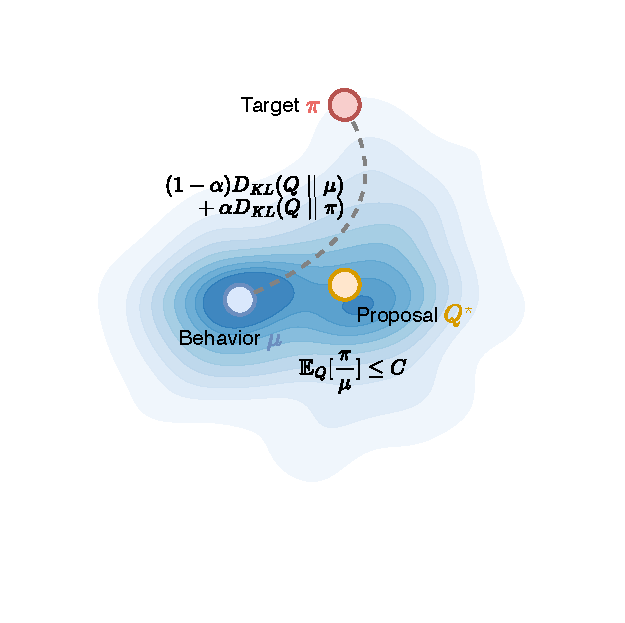
\includegraphics[width=0.45\columnwidth]{figures/overview.pdf}
  \hfill
  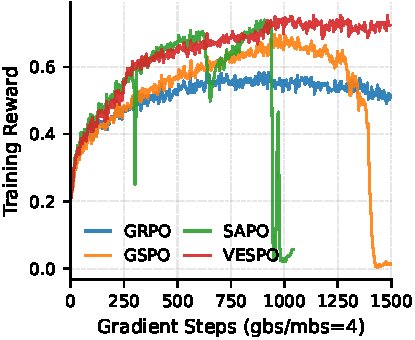
\includegraphics[width=0.53\columnwidth]{figures/overview_b.pdf}
  \caption{\textbf{左}: VESPO 将 IS 权重塑造重新表述为在方差约束下寻找一个提议 $Q^*$，使其在与 $\mu$ 和 $\pi$ 的接近性之间取得平衡。\textbf{右}: 在 Qwen3-30B-A3B-Base 上的训练奖励（gbs/mbs=4）。}
  \label{fig:overview}
\end{figure}

现有方法通过各种\emph{重要性权重变换}来应对这一挑战。大多数方法在token层面进行：GRPO~\citep{shao2024deepseekmath, DeepSeekAI2025DeepSeekR1IR}对每个token的比率应用PPO风格的截断；其他方法如SAPO~\citep{gao2025softadaptivepolicyoptimization}则为异策略重要性权重设计启发式变换~\citep{xi2025bapostabilizingoffpolicyreinforcement, zheng2025prosperity, dwyer2025itsyouitsclipping, roux2025taperedoffpolicyreinforcestable, hu2025reinforcestabilizingcriticfreepolicy}。然而，token层面的变换是一种权宜之计，旨在避免序列层面权重的乘积方差爆炸问题，且已被证明仅是其序列层面对应物的一阶近似~\citep{Zheng2025GroupSP}。序列层面的方法~\citep{Zheng2025GroupSP, zhao2025geometricmeanpolicyoptimization}引入长度规范化以控制方差，但这种规范化会使IS估计量产生有偏；仍需额外进行硬截断。尽管已有这些努力，但针对重要性权重变换设计的合理指导仍然有限。

我们提出 \textbf{V}ariational s\textbf{E}quence-level \textbf{S}oft \textbf{P}olicy \textbf{O}ptimization (\textbf{VESPO})，采用了一种根本不同的方法：与其设计重塑造启发式方法，不如将异策略重要性采样中的方差减小显式地融入变分公式中，从而得到一个有原则的闭式解 (\cref{fig:overview})。此外，我们发现所得变换特别适合序列级最优化：与以往依赖长度规范化以避免方差爆炸的方法不同，VESPO 直接在序列级重要性权重上操作，无需近似或规范化。

我们的贡献总结如下：
\begin{itemize}[itemsep=-1pt, topsep=-1pt]
  \item 我们显式地将方差减小纳入重要性权重重塑的变分公式中，并推导出一个合理的闭式解。

  \item 所得算法 \textbf{VESPO} 直接作用于序列级别的重要性权重，保留了词元间的依赖关系，同时避免了长度相关的偏差。

  \item 在数学推理基准上的实验表明，\textbf{VESPO} 在停滞比率高达 64$\times$ 以及完全异步训练下仍保持稳定，在稠密和 MoE 架构上均实现了持续的性能提升。
\end{itemize}


\section{初步研究}
\label{sec:prelim}

\textbf{符号说明.}
我们考虑一个由 $\theta$ 参数化的自回归语言模型作为策略 $\pi_\theta$。
令 $x$ 表示从数据集 $\mathcal{D}$ 中采样的查询。
在异策略情景下，响应 $y = (y_1, \ldots, y_T)$ 从行为策略 $\mu$ 中采样（例如，早期的检查点或不同的推理引擎）。
给定 $x$ 生成 $y$ 的似然可分解为：
\begin{equation}
  \label{eq:autoregressive}
  \pi_\theta(y \mid x) = \prod_{t=1}^{T} \pi_\theta(y_t \mid x, y_{<t}).
\end{equation}
我们用 $\tau = (x, y)$ 表示一个查询-响应对，用 $R(\tau) \in \mathbb{R}$ 表示分配给完整响应的序列级奖励。

\textbf{带异策略修正的策略梯度。}
目标是最大化当前策略下的期望奖励：
\begin{equation}
  \label{eq:objective}
  \mathcal{J}(\theta) = \mathbb{E}_{\tau \sim \pi_\theta}\bigl[R(\tau)\bigr].
\end{equation}
当样本从行为策略 $\mu$ 中抽取时，重要性采样提供了无偏修正。  
求梯度得到异策略策略梯度：
\begin{equation}
  \label{eq:off-policy-pg}
  \nabla_\theta \mathcal{J}(\theta) = \mathbb{E}_{\tau \sim \mu}\left[W(\tau) \cdot R(\tau) \cdot \nabla_\theta \log \pi_\theta(\tau)\right],
\end{equation}
其中 $W(\tau) = \pi_\theta(\tau) / \mu(\tau)$ 为重要性权重。  
这种经典的策略梯度视角~\cite{sutton1999policy} 揭示了重要性权重 $W$ 充当一个 \emph{梯度权重因子}：它决定了每个样本对参数更新的贡献程度。  
更一般地，对重要性权重的任何修改都可以理解为定义了一个重塑函数 $\phi(W)$，该函数重新加权梯度：
\begin{equation}
  \label{eq:reshaped-pg}
  \nabla_\theta \tilde{\mathcal{J}}(\theta) = \mathbb{E}_{\tau \sim \mu}\left[\phi(W(\tau)) \cdot R(\tau) \cdot \nabla_\theta \log \pi_\theta(\tau)\right].
\end{equation}
这种以梯度为中心的视角将贯穿我们的分析：任何权重变换的实际效果，最终都必须通过其如何重新加权策略梯度来理解。

\textbf{序列级IS的方差挑战。}
将重要性权重按token级比例展开，揭示了其基本的结构性矛盾。
定义token级重要性比率为 $\rho_t = \frac{\pi_\theta(y_t \mid x, y_{<t})}{\mu(y_t \mid x, y_{<t})}$ 。
则序列级权重为一个乘积：
\begin{equation}
  \label{eq:seq-weight}
  W(\tau) = \prod_{t=1}^{T} \rho_t,
\end{equation}
而对数策略梯度则是一个求和：
\begin{equation}
  \label{eq:log-grad-sum}
  \nabla_\theta \log \pi_\theta(\tau) = \sum_{t=1}^{T} \nabla_\theta \log \pi_\theta(y_t \mid x, y_{<t}).
\end{equation}
这种乘积-求和结构产生了一种张力：每个 token 的梯度贡献被一个全局因子 $W(\tau)$ 加权，并在所有 $T$ 位置上累积。  
即使每个 token 的偏差很小，也会以乘法方式累积，导致长序列中 $W(\tau)$ 出现极端值。  
$W$ 的方差随 $T$ 呈指数增长，使得朴素的重要性采样变得不切实际。

为了抑制这种方差，现有方法定义了特定的塑造函数 $\phi$ ，用于调整梯度权重。  
GRPO~\citep{shao2024deepseekmath} 在 token 级别上操作，采用类似 PPO 的截断代理函数。  
从梯度的角度来看，有效权重函数取决于优势 $A$ 的符号：
\begin{equation}
  \label{eq:grpo-phi}
  \phi_{\text{GRPO}}(\rho_t; A) =
  \begin{cases}
    \rho_t, & \text{if } A > 0 \text{ and } \rho_t \leq 1{+}\varepsilon, \\
    \rho_t, & \text{if } A < 0 \text{ and } \rho_t \geq 1{-}\varepsilon, \\
    0,      & \text{otherwise (gradient zeroed)}.
  \end{cases}
\end{equation}
这破坏了乘积结构，将每个 token 更新独立处理，仅得到一阶近似~\citep{Zheng2025StabilizingRL}。

GSPO~\citep{Zheng2025GroupSP} 在序列层面操作，将梯度权重定义为 token 级别比率的几何平均值（即通过序列长度进行归一化）：
\begin{equation}
  \label{eq:gspo-phi}
  \phi_{\text{GSPO}}(W) = \left(\prod_{t=1}^{T} \rho_t\right)^{\!1/T} = \exp\left(\frac{1}{T}\sum_{t=1}^{T}\log\rho_t\right),
\end{equation}
随后采用类似于GRPO的裁剪机制。  
这种规范化引入了与长度相关的偏差：隐式的提议分布随 $T$ 变化，即使不同长度的序列具有相同的每token统计量，它们也会获得相同的权重，尽管其真实的重要的权重不同（详见 \cref{app:length-normalization} 的形式化分析）。  
这些方法均对 $\phi$ 进行启发式定义；何为 $\phi$ 的合理选择这一问题，正是我们接下来所发展的变分框架所要解决的核心。


\section{VESPO：变分序列级软策略最优化}
\label{sec:vespo}

我们提出一个设计重要性权重变换的合理框架。首先，我们证明了任意的重塑函数 $\phi(W)$  隐式地定义了一个提议分布，然后将 $\phi$  的设计表述为带有方差约束的变分问题，并最终推导出闭式解。

\subsection{权重重塑作为测度变换}
\label{sec:measure-change}

标准重要性采样执行一个无偏的测度变换 $\mu \to \pi$ ，而任何变换 $\phi(W)$ 会对某个隐含的提议分布 $Q$ 引入不同的测度变换 $\mu \to Q$ 。  
我们现在对这一观点进行形式化。  
对于任意函数 $G(\tau)$ ：
\begin{equation}
  \label{eq:measure-change}
  \mathbb{E}_{\tau \sim \mu}\bigl[\phi(W(\tau)) \cdot G(\tau)\bigr] = Z \cdot \mathbb{E}_{\tau \sim Q}\bigl[G(\tau)\bigr],
\end{equation}
其中 $Z = \mathbb{E}_{\mu}[\phi(W)]$ 为规范化常数，$Q$ 由下式定义
\begin{equation}
  \label{eq:proposal-def}
  Q(\tau) = \frac{1}{Z} \mu(\tau) \cdot \phi(W(\tau)).
\end{equation}
重排后的梯度 (\cref{eq:reshaped-pg}) 在标量 $Z$ 的意义下，等价于提议分布 $Q$ 下的同策略梯度。

这是关键的洞察：任何序列级的塑造函数 $\phi(W)$  隐式地定义了一个提议分布 $Q$ 。  
这一视角提供了一个统一的透镜来分析现有的重要性权重变换（详见 \cref{app:implicit-proposals} 对具体方法的详细分析）。  
我们不需要直接设计 $\phi$ ，而是可以指定提议 $Q$ 的期望属性，并推导出相应的 $\phi$ 。  
一个好的提议应尽可能接近 $\mu$ 以提高采样效率，融入 $\pi$ 以指导最优化，并控制方差。  
以下小节将这些期望属性形式化为一个变分目标，并推导出闭式 $\phi^*$ 。

\subsection{变分目标}
\label{sec:variational-objective}

\textbf{双重邻近性。}
我们寻求一个提议 $Q$，使其在样本效率方面保持与 $\mu$ 的接近，同时向 $\pi$ 靠近以降低估计偏差。
我们通过一种混合KL目标来形式化这一思想，该目标促使 $Q$ 在分布空间中位于 $\mu$ 与 $\pi$ 之间：
\begin{equation}
  \label{eq:dual-kl}
  \mathcal{J}(Q) = (1-\alpha) \, D_{\mathrm{KL}}(Q \| \mu) + \alpha \, D_{\mathrm{KL}}(Q \| \pi),
\end{equation}
其中 $\alpha$ 控制权衡。  
第一项惩罚与采样分布的偏离，确保从 $\mu$ 采样的样本在估计 $Q$ 下的期望时保持信息量。  
第二项惩罚与目标策略的偏离，降低梯度估计的偏差。

\textbf{方差约束。}
仅考虑接近性是不够的：有限样本大小要求对方差进行控制。
在重要性采样中，估计量的方差与二阶矩 $\mathbb{E}_\mu[W^2]$ 成比例，这是一个经典结果，同时也构成了有效样本大小（ESS）诊断的基础。

在测度变换视角下，这个二阶矩可以与 $Q$ 下的一个期望相关联。根据 \cref{eq:proposal-def}，我们有 $Q(\tau) \propto \mu(\tau) \phi(W(\tau))$，因此
\begin{equation}
  \label{eq:variance-link}
  \mathbb{E}_{\tau \sim Q}[W(\tau)] \propto \mathbb{E}_{\tau \sim \mu}[\phi(W) \cdot W].
\end{equation}
当 $\phi(W) \approx W$  （趋近于无偏IS）时，这恢复了 $\mathbb{E}_\mu[W^2]$ 。因此，对 $\mathbb{E}_Q[W]$ 进行边界限定提供了一种有原则的方法来控制由测度变化引起的方差：
\begin{equation}
  \label{eq:moment-constraint}
  \mathbb{E}_{\tau \sim Q}[W(\tau)] \leq C.
\end{equation}

\textbf{约束优化。}
将双邻近目标与方差约束相结合：
\begin{align}
  \label{eq:constrained-opt}
  \min_{Q} \;    & (1-\alpha) \, D_{\mathrm{KL}}(Q \| \mu) + \alpha \, D_{\mathrm{KL}}(Q \| \pi) \notag \\
  \text{s.t.} \; & \mathbb{E}_{Q}[W] \leq C, \quad \textstyle\int Q = 1.
\end{align}
引入拉格朗日乘子 $\lambda \geq 0$ 用于时刻约束，以及 $\gamma$ 用于规范化，我们得到拉格朗日函数：
\begin{align}
  \label{eq:lagrangian}
  \mathcal{L}(Q, \lambda, \gamma) = \; & (1{-}\alpha) D_{\mathrm{KL}}(Q \| \mu) + \alpha D_{\mathrm{KL}}(Q \| \pi) \notag         \\
                                       & + \lambda \bigl(\mathbb{E}_Q[W] {-} C\bigr) + \gamma \bigl(\textstyle\int Q {-} 1\bigr).
\end{align}

\subsection{闭式解}
\label{sec:closed-form}

对泛函导数 $\frac{\delta \mathcal{L}}{\delta Q} = 0$ 取导数得到（见 \cref{app:variational-derivation}）：
\begin{equation}
  \label{eq:Q-solution}
  Q^*(\tau) \propto \mu(\tau)^{1-\alpha} \, \pi(\tau)^{\alpha} \, \exp(-\lambda W(\tau)).
\end{equation}
使用 $W = \pi/\mu$，这简化为 $Q^*(\tau) \propto \mu(\tau) \cdot W(\tau)^{\alpha} \cdot \exp(-\lambda W(\tau))$。  
与 \cref{eq:proposal-def} 比较，我们确定了重塑函数：
\begin{equation}
  \label{eq:gamma-kernel}
  \phi(W) = W^{\alpha} \cdot \exp(-\lambda W).
\end{equation}

该核函数包含两个部分：用于软抑制的幂次项 $W^\alpha$  和指数项 $\exp(-\lambda W)$ 。  
它在所有位置都光滑且可微，避免了硬裁剪带来的不连续性。

\textbf{代理目标解释。}
回顾一下，我们的目标是最大化期望奖励 $\mathcal{J}(\theta) = \mathbb{E}_{\tau \sim \pi_\theta}[R(\tau)]$  (\cref{eq:objective})。
利用来自 $\mu$ 的异策略样本，重塑后的梯度 (\cref{eq:reshaped-pg}) 可以看作是在优化一个代理目标。
注意到 $\nabla_\theta W = W \nabla_\theta \log \pi_\theta$ ，因此梯度估计量可以重写为
\begin{equation}
  \label{eq:grad-rewrite}
  \mathbb{E}_{\tau \sim \mu}[\phi(W) \cdot A \cdot \nabla \log \pi_\theta] = \mathbb{E}_{\tau \sim \mu}\bigl[\tfrac{\phi(W)}{W} \cdot A \cdot \nabla W\bigr].
\end{equation}
定义 $f(W)$ 使得 $f'(W) = \phi(W)/W$ ，右边等于 $\nabla_\theta \mathbb{E}_{\tau \sim \mu}[f(W) \cdot A]$ ，因为 $A(\tau)$ 不依赖于 $\theta$ 。  
因此，VESPO 隐式地最大化一个代理目标：
\begin{equation}
  \label{eq:surrogate-obj}
  \mathcal{J}_{\text{VESPO}}(\theta) = \mathbb{E}_{\tau \sim \mu}\bigl[f(W(\theta)) \cdot A(\tau)\bigr].
\end{equation}
对于 $\phi(W) = W^\alpha \exp(-\lambda W)$ ，我们有 $f'(W) = W^{\alpha-1} \exp(-\lambda W)$ ，其积分结果为 \emph{下不完全伽马函数}：
\begin{equation}
  \label{eq:f-gamma}
  f(W) = \frac{1}{\lambda^\alpha} \, \gamma(\alpha, \lambda W), \quad \text{where } \gamma(a, x) = \int_0^x t^{a-1} e^{-t} \, dt.
\end{equation}
此形式光滑且无限可微，当 $W \to \infty$ 时趋于饱和，为硬削波提供了一种合理的软替代方案。

\begin{figure}[t]
  \centering
  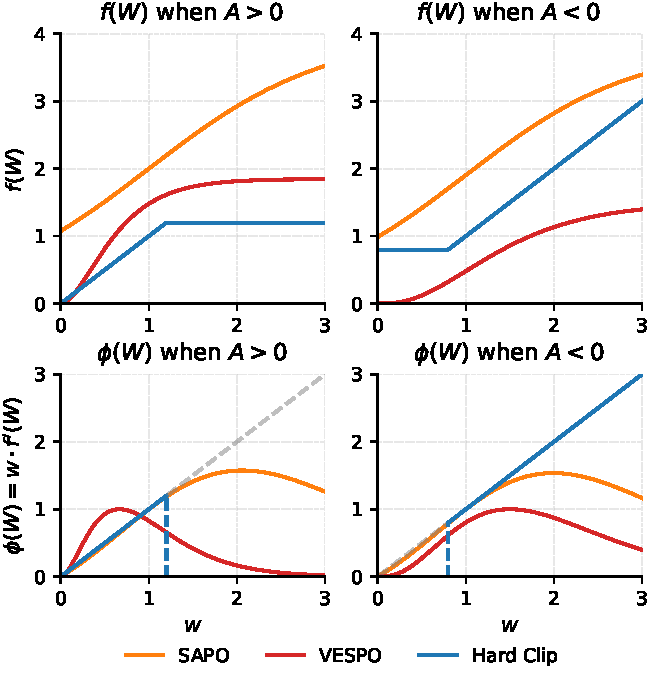
\includegraphics[width=\columnwidth]{figures/phi_and_f_comparison.pdf}
  \caption{代理目标 $f(w)$ （上）和梯度缩放因子 $\phi(w) = w \cdot f'(w)$ （下）对于正优势和负优势。硬截断在边界处突然将 $\phi$ 置零；VESPO 在 $w{=}1$ 附近达到峰值并平滑衰减。}
  \label{fig:phi-comparison}
\end{figure}

\subsection{VESPO算法}
\label{sec:vespo-algorithm}

在实际应用中，我们使用平移形式 $\phi(W) = W^{c_1} \exp(c_2(1 - W))$ 以确保 $\phi(1) = 1$ ，从而使同策略样本获得单位权重，且更新幅度在相同学习率下与标准同策略方法保持一致。  
我们为正向和负向优势采用不同的超参数 $(c_1, c_2)$ ，以模仿 PPO 中的非对称裁剪机制。  
近期工作~\citep{tang2025rethinkingsamplepolarityreinforcement} 表明，训练过程中正负样本表现出不同的梯度动态；因此，我们对 $A < 0$ 采用更强的抑制策略，通过 $W < 1$ 防止对策略已不喜好的样本施加过度惩罚，如 \cref{fig:phi-comparison} 所示。  
我们将 $(c_1, c_2)$ 视为可调节的超参数，从而在变分推导所隐含的具体取值之外提供更大的灵活性。  
将平移核代入 \cref{eq:reshaped-pg} 后，VESPO 估计量变为：
\begin{align}
  \label{eq:vespo-gradient}
  \nabla \mathcal{J}_{\text{VESPO}} = \mathbb{E}_{\tau \sim \mu}\bigl[ & W^{c_1} \exp(c_2(1 {-} W)) \notag                        \\
                                                                       & \cdot A(\tau) \cdot \nabla \log \pi_\theta(\tau) \bigr],
\end{align}
其中 $A(\tau) = R(\tau) - b$  是带有基准 $b$ 的优势值（按每个提示组内的平均奖励计算，遵循 GRPO~\citep{shao2024deepseekmath}）。

\textbf{与现有方法的联系。}
核函数表现出自适应特性：当 $W \approx 1$ 时，$\phi(W) \approx 1$ 和梯度得以保留；当 $W \gg 1$ 时，指数项迅速衰减；当 $W \ll 1$ 时，幂项自然地对不太可能的样本进行降权。
相较于硬截断，VESPO 提供了一种平滑的近似，能够渐进地衰减极端权重 (\cref{fig:phi-comparison})。
相较于现有的在 token 级别操作的软变换，VESPO 直接应用于序列级重要性权重，无需长度规范化，且分解形式提供了灵活的控制：$c_1$ 主要控制 $W < 1$ 时的行为，而 $c_2$ 则调控 $W > 1$ 时的衰减。

\textbf{实现。}
我们将 VESPO 以 REINFORCE 风格实现：重塑权重 $\phi(W)$ 从计算图中分离，仅作为梯度缩放系数。
序列级重要性权重在对数空间中计算，以保证数值稳定性：
\begin{equation}
  \label{eq:log-weight}
  \log W = \sum_{t=1}^{T} \bigl( \log \pi_\theta(y_t | x, y_{<t}) - \log \mu(y_t | x, y_{<t}) \bigr).
\end{equation}
重塑 $c_1 \log W + c_2(1-W)$  也在对数空间中计算；仅在最后一步进行指数运算，从而避免极端重要性权重导致的上溢。  
这只需要存储在 $\pi$  和 $\mu$  下每个 token 的对数概率，无需额外的内存开销。  
完整的伪代码见 \cref{app:algorithm}。



\section{实验}
\label{sec:experiments}

我们在数学推理基准上评估 VESPO，重点关注异策略分布偏移的实际来源：(1) \textbf{策略滞后的} 问题，源于批量回放，其中后期的小批量使用过时策略的样本进行更新，包括一种完全异步的情景，即回放和训练在分离的结点上运行；以及 (2) \textbf{训练-推理不匹配}，即训练与推理引擎之间不同的实现导致相同输入产生不同输出——这一现象在 MoE 模型中由于路由不一致而被加剧。

\subsection{实验设置}
\label{sec:exp-setup}

\textbf{训练。}
所有实验均在 32 块 NVIDIA H20 GPU 上使用 veRL 框架~\citep{sheng2024hybridflow} 进行，推理采用 vLLM 0.11.0~\citep{kwon2023efficient}，稠密模型的训练使用 FSDP~\citep{zhao2023pytorch}（MoE 使用 Megatron~\citep{shoeybi2019megatron}）。
训练数据集为未过滤的 DAPO-Math~\citep{yu2025dapo} 版本，该数据集提供了足够的训练数据以支持更长时间的训练。
对于每个查询，我们采样 8 个响应，并使用 Math-Verify~\citep{mathverify2025} 计算奖励。
我们将训练和评估的最大上下文长度设置为 16,384 token。
所有方法均训练 1,500 个梯度步数。更多细节见~\cref{tab:hyperparams}。

\textbf{模型。}
我们在三个模型规模上进行评估：Llama-3.2-3B-Instruct~\citep{grattafiori2024llama3herdmodels}、Qwen3-8B-Base，以及 Qwen3-30B-A3B-Base~\citep{Yang2025Qwen3TR}。
MoE 架构由于路由决策在各层间累积，加剧了训练-推理不匹配问题。

\textbf{评估。}
我们在四个数学推理基准上进行评估：AIME 2024、AIME 2025、AMC 2023 和 MATH-500~\citep{hendrycks2021measuring}。
我们报告 avg@$k$ 准确率（对每个问题的 $k$ 个采样响应取平均），其中 AIME 2024/2025 使用 $k=32$，AMC 2023 使用 $k=16$，MATH-500 使用 $k=4$。
我们根据在所有四个基准上的平均表现选择最佳检查点。

\textbf{基准.}
我们与三种代表性方法进行对比：
{GRPO}~\citep{shao2024deepseekmath}，该方法在 token 级别应用 PPO 风格的裁剪，裁剪比例 $(0.2, 0.28)$ 依照 DAPO~\citep{yu2025dapo}；
{GSPO}~\citep{Zheng2025GroupSP}，该方法在序列级别操作，采用 $1/T$  长度规范化和裁剪比例 $(3\text{e-}4, 4\text{e-}4)$；
以及 {SAPO}~\citep{gao2025softadaptivepolicyoptimization}，该方法使用软自适应门控，其中 $\tau_{\text{pos}}=1.0$  和 $\tau_{\text{neg}}=1.05$。
对于 VESPO，我们使用 $(c_1, c_2) = (2.0, 3.0)$  作为 $A > 0$  以及 $(c_1, c_2) = (3.0, 2.0)$  作为 $A < 0$。

为了模拟策略陈旧性，我们将小批量大小（mbs）固定为256，并通过改变全局批量大小（gbs）来控制异策略更新的程度。  
当 gbs/mbs $= N$ 时，每次生成的 gbs 个样本会被拆分为 $N$ 个小批量，用于顺序的策略梯度更新。  
我们通过策略更新步数来衡量进展，以确保所有方法处理的数据量相同。  
我们的主要实验使用 $N = 8$ ，而消融实验则探索 $N \in \{4, 8, 16, 32, 64\}$ 。

我们还在一个完全异步的情景下进行评估，其中采样和训练在分离的结点组上运行。  
训练器每4次本地更新就将更新后的权重同步到采样引擎（类似于同步情景下的 gbs/mbs${=}4$），并且在同步边界之间保留由过时参数生成的飞行中采样结果，而非丢弃~\citep{zhou2025april}。

\subsection{主要结果}
\label{sec:main-results}

\begin{table}[h]
  \caption{数学推理准确率（\%）随 gbs/mbs $= 8$ 变化。我们报告 AIME24/25 的 avg@32，AMC23 的 avg@16，以及 MATH500 的 avg@4。每种模型的最佳结果以 \textbf{粗体} 标出。}
  \label{tab:main-results}
  \centering
  \begin{small}
    \setlength{\tabcolsep}{1.0pt}
    \begin{tabular}{@{}l|l|ccccc@{}}
      \toprule
      Model & Method                        & AIME25                                & AIME24                                & AMC23                                 & MATH500                               & Avg                                   \\
      \midrule
      \multirow{4}{*}{\makecell[l]{Llama-                                                                                                                                                                                                           \\3.2-3B-\\Instruct}}
            & GRPO                          & 0.5                                   & {14.5}                                & 40.6                                  & 43.8                                  & 24.8                                  \\
            & GSPO                          & 0.2                                   & \textbf{14.7}                         & 43.9                                  & 41.4                                  & 25.1                                  \\
            & SAPO                          & \textbf{0.7}                          & 12.2                                  & 34.1                                  & 41.3                                  & 22.1                                  \\
            & \cellcolor{ourhighlight}VESPO & \cellcolor{ourhighlight}0.6           & \cellcolor{ourhighlight}13.9          & \cellcolor{ourhighlight}\textbf{47.3} & \cellcolor{ourhighlight}\textbf{45.3} & \cellcolor{ourhighlight}\textbf{26.8} \\
      \midrule
      \multirow{4}{*}{\makecell[l]{Qwen3-                                                                                                                                                                                                           \\8B-Base}}
            & GRPO                          & 27.4                                  & 40.0                                  & 74.5                                  & 68.6                                  & 52.6                                  \\
            & GSPO                          & 28.8                                  & 37.7                                  & 80.8                                  & 70.4                                  & 54.4                                  \\
            & SAPO                          & \textbf{36.7}                         & {49.0}                                & 80.0                                  & 70.3                                  & 59.0                                  \\
            & \cellcolor{ourhighlight}VESPO & \cellcolor{ourhighlight}{33.5}        & \cellcolor{ourhighlight}\textbf{49.4} & \cellcolor{ourhighlight}\textbf{82.2} & \cellcolor{ourhighlight}\textbf{71.1} & \cellcolor{ourhighlight}\textbf{59.0} \\
      \midrule
      \multirow{4}{*}{\makecell[l]{Qwen3-                                                                                                                                                                                                           \\30B-A3B-\\Base}}
            & GRPO                          & 28.2                                  & 40.0                                  & \textbf{81.4}                         & 69.9                                  & 54.9                                  \\
            & GSPO                          & 24.6                                  & 34.1                                  & 80.5                                  & 68.8                                  & 52.0                                  \\
            & SAPO                          & 21.4                                  & 27.9                                  & 73.0                                  & 68.7                                  & 47.7                                  \\
            & \cellcolor{ourhighlight}VESPO & \cellcolor{ourhighlight}\textbf{34.2} & \cellcolor{ourhighlight}\textbf{44.1} & \cellcolor{ourhighlight}80.3          & \cellcolor{ourhighlight}\textbf{70.2} & \cellcolor{ourhighlight}\textbf{57.2} \\
      \bottomrule
    \end{tabular}
  \end{small}
\end{table}

\begin{table}[t]
  \caption{不同延迟比例 $N$  (gbs/mbs) 对 Qwen3-30B-A3B-Base 的影响。我们报告 avg@$k$  (\%)。VESPO 在所有 $N$  值下均保持强劲性能。}
  \label{tab:staleness}
  \centering
  \begin{small}
    \setlength{\tabcolsep}{3.5pt}
    \begin{tabular}{@{}c|l|ccccc@{}}
      \toprule
      $N$ & Method                        & AIME25                                & AIME24                                & AMC23                                 & MATH500                               & Avg                                   \\
      \midrule
      \multirow{4}{*}{4}
          & GRPO                          & 22.1                                  & 33.1                                  & 76.4                                  & 67.7                                  & 49.8                                  \\
          & GSPO                          & 27.6                                  & 43.3                                  & 83.1                                  & 70.4                                  & 56.1                                  \\
          & SAPO                          & 38.4                                  & 51.4                                  & 85.2                                  & \textbf{71.2}                         & 61.5                                  \\
          & \cellcolor{ourhighlight}VESPO & \cellcolor{ourhighlight}\textbf{43.1} & \cellcolor{ourhighlight}\textbf{60.3} & \cellcolor{ourhighlight}\textbf{91.2} & \cellcolor{ourhighlight}71.1          & \cellcolor{ourhighlight}\textbf{66.4} \\
      \midrule
      \multirow{4}{*}{8}
          & GRPO                          & 28.2                                  & 40.0                                  & 81.4                                  & 69.9                                  & 54.9                                  \\
          & GSPO                          & 25.1                                  & 43.3                                  & 83.0                                  & 69.6                                  & 55.3                                  \\
          & SAPO                          & 21.4                                  & 27.9                                  & 73.0                                  & 68.7                                  & 47.7                                  \\
          & \cellcolor{ourhighlight}VESPO & \cellcolor{ourhighlight}\textbf{44.3} & \cellcolor{ourhighlight}\textbf{59.6} & \cellcolor{ourhighlight}\textbf{91.4} & \cellcolor{ourhighlight}\textbf{72.4} & \cellcolor{ourhighlight}\textbf{66.9} \\
      \midrule
      \multirow{4}{*}{16}
          & GRPO                          & 20.3                                  & 31.4                                  & 71.4                                  & 67.9                                  & 47.7                                  \\
          & GSPO                          & 24.3                                  & 41.6                                  & 83.1                                  & 71.4                                  & 55.1                                  \\
          & SAPO                          & 19.6                                  & 26.0                                  & 72.2                                  & 68.0                                  & 46.5                                  \\
          & \cellcolor{ourhighlight}VESPO & \cellcolor{ourhighlight}\textbf{40.2} & \cellcolor{ourhighlight}\textbf{53.2} & \cellcolor{ourhighlight}\textbf{90.8} & \cellcolor{ourhighlight}\textbf{71.5} & \cellcolor{ourhighlight}\textbf{63.9} \\
      \midrule
      \multirow{4}{*}{32}
          & GRPO                          & 21.8                                  & 33.4                                  & 73.4                                  & 68.3                                  & 49.2                                  \\
          & GSPO                          & 18.8                                  & 27.3                                  & 73.4                                  & {70.6}                                & 47.5                                  \\
          & SAPO                          & 12.4                                  & 7.2                                   & 29.5                                  & 30.2                                  & 19.8                                  \\
          & \cellcolor{ourhighlight}VESPO & \cellcolor{ourhighlight}\textbf{37.7} & \cellcolor{ourhighlight}\textbf{51.4} & \cellcolor{ourhighlight}\textbf{85.2} & \cellcolor{ourhighlight}\textbf{71.3} & \cellcolor{ourhighlight}\textbf{61.4} \\
      \midrule
      \multirow{4}{*}{64}
          & GRPO                          & 14.6                                  & 28.0                                  & 69.4                                  & 66.8                                  & 44.7                                  \\
          & GSPO                          & 15.4                                  & 24.1                                  & 73.9                                  & \textbf{70.0}                         & 45.8                                  \\
          & SAPO                          & 3.3                                   & 7.3                                   & 23.8                                  & 39.4                                  & 18.4                                  \\
          & \cellcolor{ourhighlight}VESPO & \cellcolor{ourhighlight}\textbf{34.2} & \cellcolor{ourhighlight}\textbf{46.2} & \cellcolor{ourhighlight}\textbf{83.6} & \cellcolor{ourhighlight}69.9          & \cellcolor{ourhighlight}\textbf{58.5} \\
      \bottomrule
    \end{tabular}
  \end{small}
  \vspace{-1em}
\end{table}


\cref{tab:main-results} 展示了在三个模型规模下，gbs/mbs $= 8$ 的主要结果。  
VESPO 在所有三个模型上均取得了最佳的平均准确率，展现了我们方法的通用性。  
值得注意的是，在 Qwen3-30B-A3B-Base 上，性能提升最为显著，VESPO 相比最佳基准提升了 2.3\% 的平均准确率。  
这表明，VESPO 对极端重要性权重的软抑制机制对 MoE 架构尤为有益，因为在这些架构中，路由不一致会加剧分布偏移，使训练稳定性更难维持。  
基于上述观察，我们在后续章节中将重点分析 Qwen3-30B-A3B-Base 模型。

\subsection{策略迟滞的鲁棒性}
\label{sec:staleness}

\begin{figure}[t]
  \centering
  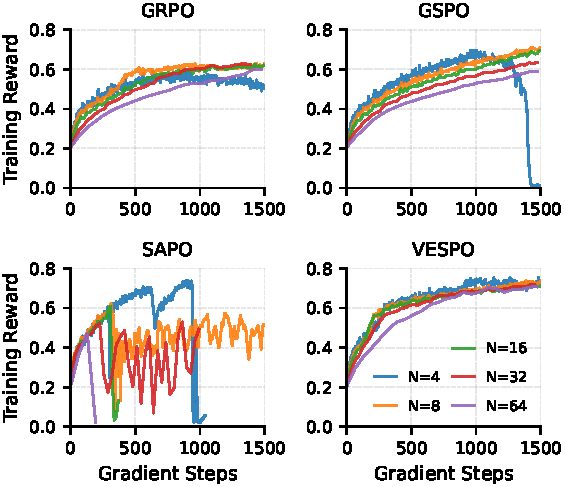
\includegraphics[width=\columnwidth]{figures/training_dynamics_2x2.pdf}
  \caption{不同延迟级别 ($N \in \{4, 8, 16, 32, 64\}$ ) 下 Qwen3-30B-A3B-Base 的训练奖励。每个面板显示一种方法在不同 $N$ 值下的表现。VESPO 在所有延迟级别下均保持稳定且一致的训练曲线。
  }
  \label{fig:training-reward-comparison}
  \vspace{-1em}
\end{figure}

我们通过将策略陈旧率 $N = \text{gbs}/\text{mbs}$ 从 4 变化到 64 来检验对策略陈旧的鲁棒性。  
\cref{fig:training-reward-comparison} 提供了不同方法在训练稳定性方面的直接对比。  
VESPO 展现出显著的一致性：五条曲线（$N{=}4$ 到 $N{=}64$）几乎遵循相同的轨迹，收敛至约 0.7 的相似最终奖励，对策略陈旧表现出极小的敏感性。  
相比之下，GRPO 在次优奖励水平上早期饱和，且随着 $N$ 增大，收敛速度变慢。  
GSPO 显示出陈旧性与最终性能之间的明显相关性：更大的 $N$ 导致更低的收敛奖励。在 $N{=}4$ 时，GSPO 在第 1,200 步左右出现灾难性崩溃，奖励降至零。  
SAPO 在 $N{=}4$ 时表现出不稳定的训练，在 $N{\geq}8$ 时完全崩溃，这一模式将在下文与 \cref{fig:phi-comparison} 进一步分析。  
这些训练动态的差异直接转化为下游性能的差异，如 \cref{tab:staleness} 所示：  
在每个 gbs/mbs 情景下，VESPO 均取得最佳平均准确率，并在 $N{=}64$ 时仍保持强劲表现；而 GRPO 和 GSPO 分别退化至 44.7\% 和 45.8\%，SAPO 则回落至基准水平（18.4\%）。

\begin{figure*}[t]
  \centering
  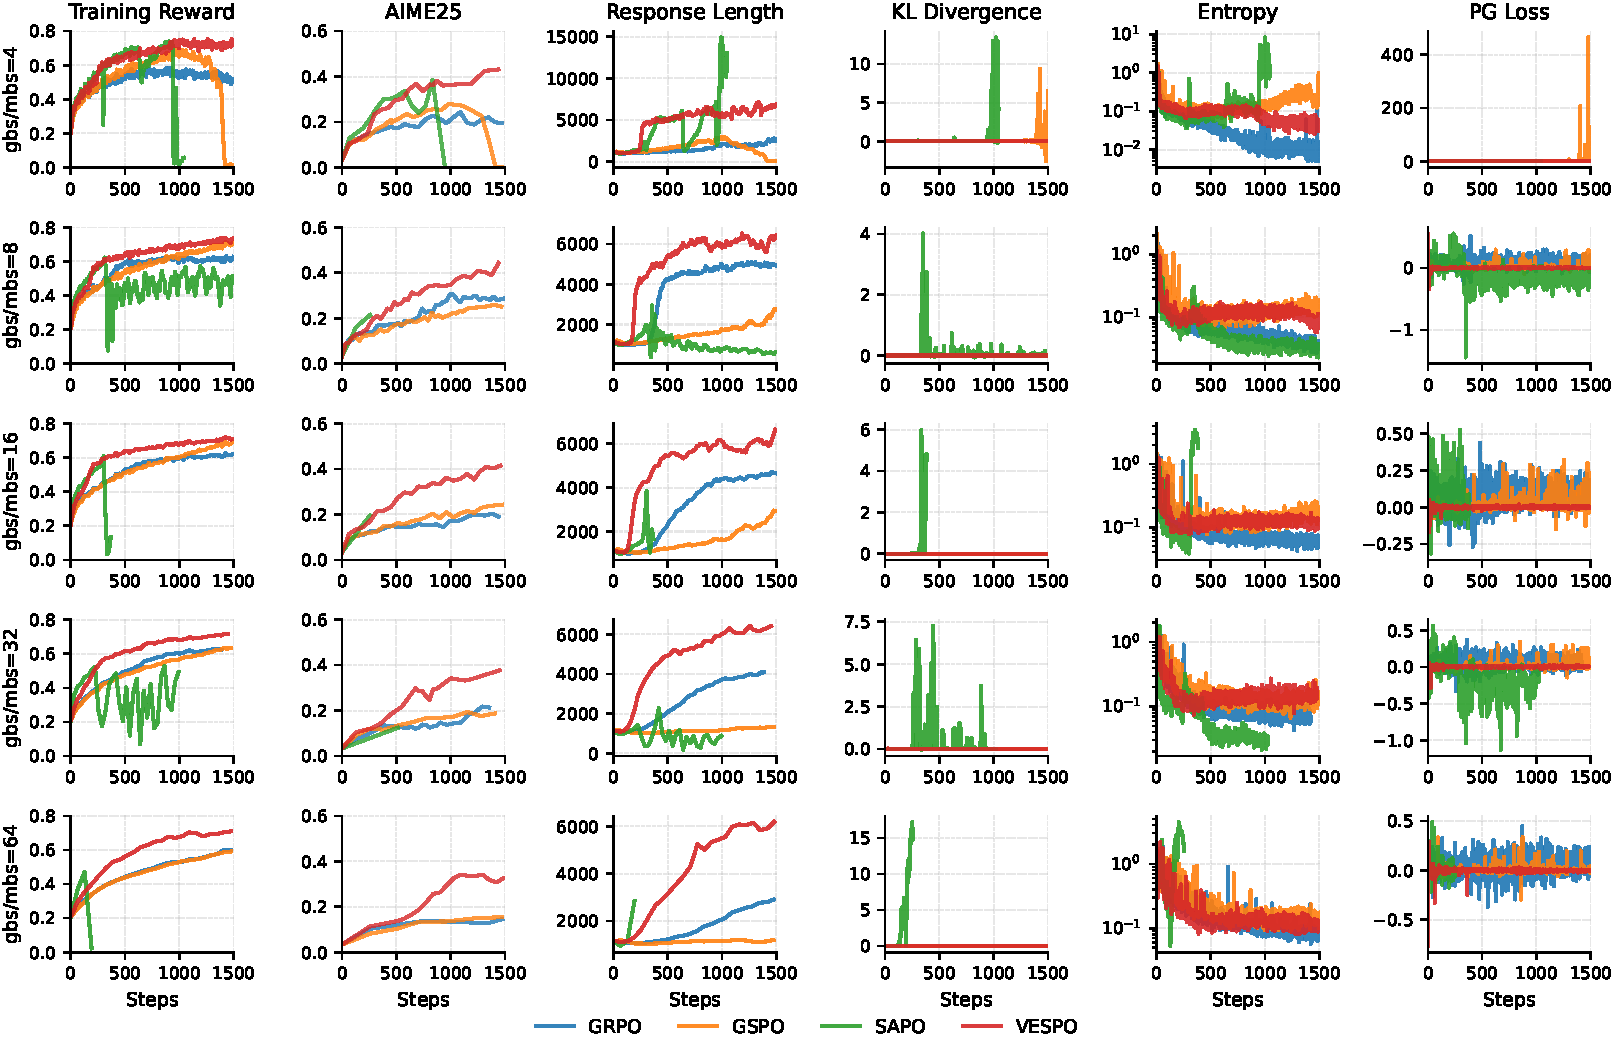
\includegraphics[width=\textwidth]{figures/training_dynamics_5x6.pdf}
  \caption{不同延迟等级下的训练动态 ($N$  = gbs/mbs $\in \{4, 8, 16, 32, 64\}$ ) 在 Qwen3-30B-A3B-Base 上的表现。每一行对应不同的 $N$；列展示了训练奖励、AIME25 准确率、响应长度、KL 散度、熵和 PG 损失。VESPO（红色）在所有条件下均保持稳定的训练，而基线方法则表现出典型的失败模式。}
  \label{fig:training-dynamics}
  \vspace{-.6em}
\end{figure*}

\textbf{训练动态分析。}
\cref{fig:training-dynamics} 从六个指标全面展示了训练动态（注：y轴为响应长度，各行的刻度不同），揭示了每种方法的独特模式（详见 \cref{app:failure-modes} 的附加可视化）。

\emph{GRPO} 在所有 $N$  值下均在次优奖励水平处提前饱和。熵列显示熵值迅速下降，在发现高奖励行为之前限制了探索。

\emph{GSPO} 表现出长度偏差放大现象。  
在 $N{=}4$ 时，响应长度在接近 1,200 步前达到近 3,000 个 token 的峰值，随后发生灾难性崩溃。  
$1/T$  规范化使得较长序列更不容易被截断（\cref{app:length-normalization}）；结合 token 求和损失聚合，这会形成一个反馈环，使模型倾向于生成更长的输出。

\emph{SAPO} 显示出快速的响应长度增长，在早期训练中，在 $N{=}4$ 时达到了最多 15k tokens。

As shown in \cref{fig:phi-comparison}, SAPO的设计对于带有 $\rho_t {<}1$ 的负优势样本缺乏足够的下调权重，导致过度惩罚。

这与最近的观察一致，即负优势样本会导致长度爆炸和训练崩溃~\citep{tang2025rethinkingsamplepolarityreinforcement}。

\emph{VESPO} 在所有指标上均表现出稳定的性能。  
基准得分在训练过程中持续提升；熵值保持在稳定且相对较高的水平；响应长度维持在约 5--6k token，表明仍有进一步缩放的空间；且在所有 $N$ 取值下，PG 损失均表现出显著的稳定性。


\textbf{完全异步训练。}
上述实验通过改变 $N$ ，在同步框架内模拟了延迟现象。
我们进一步在 \cref{sec:exp-setup} 描述的完全异步情景下进行评估，其中行为策略可落后于训练策略多个梯度更新。

\begin{figure*}[ht]
  \centering
  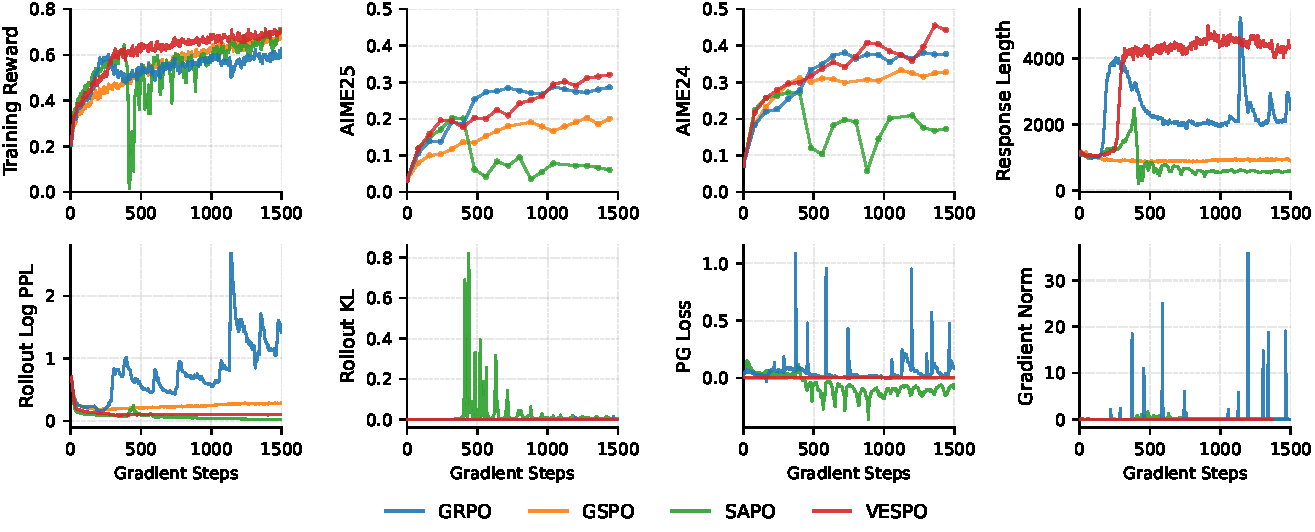
\includegraphics[width=\textwidth]{figures/fully_async_2x4.pdf}
  \caption{在Qwen3-30B-A3B-Base上的完全异步训练动态中，VESPO保持了稳定的训练过程，并达到了最高的奖励和基准准确率。}
  \vspace{-1.0em}
  \label{fig:fully-async}
\end{figure*}

\cref{fig:fully-async} 展示了该情景下的训练动态。SAPO 早期崩溃，与同步设置下的不稳定性一致。GRPO 表现出高度不稳定的训练过程：滚动采样困惑度上升至 2.0 以上，PG 损失和梯度范数频繁出现大幅波动，响应长度剧烈振荡，表明过时的滚动采样严重干扰了梯度估计。GSPO 保持稳定，但收敛到较低的训练奖励和准确率。VESPO 在整个过程中维持稳定训练：滚动采样 KL 散度、困惑度、PG 损失和梯度范数均接近零且方差极小，同时实现了最高的训练奖励以及最强的 AIME25 和 AIME24 准确率，验证了其在真实异步训练情景下的鲁棒性。


\subsection{训练与推理不匹配的鲁棒性}
\label{sec:train-infer-mismatch}


除了策略过时之外，第二个异策略偏差的来源是 \emph{训练-推理不匹配}：训练（例如，FSDP/Megatron）和推理（例如，vLLM/SGLang~\citep{zheng2024sglang}）引擎之间的不同数值实现会导致相同输入产生略有不同的输出。  
这一效应在 MoE 模型中被放大，因为路由决策会跨层累积，微小的数值差异可能导致完全不同的专家分配。

两种工程技巧被提出以在存在此类不匹配的情况下稳定训练：
{截断重要性采样（TIS）}~\citep{liu-li-2025-rl-collapse} 在重要性比率表明显著发散时，将 token 级别梯度置零；
{路由重放（R2）}~\citep{ma2025stabilizingmoereinforcementlearning} 在使用训练引擎重新计算对数概率时记录路由器分配，确保在整个训练过程中专家选择的一致性。

\cref{fig:train-infer-mismatch} 比较了 Qwen3-30B-A3B-Base 上的训练稳定性。  
在不匹配条件下，原始 GRPO 表现不佳，训练奖励在约 0.60 处达到平台期。加入 TIS 或 R2 可提升 GRPO 的稳定性和最终奖励。  
值得注意的是，VESPO \emph{无需任何专门修复} 即可维持与 GRPO+R2 相当的稳定训练，表明对极端重要性权重的软抑制有助于容忍由不匹配引起的分布偏移。

此外，VESPO可与R2结合以获得额外收益：VESPO+R2在所有变体中实现了最高的训练奖励和最佳的AIME25准确率。这表明VESPO与R2、TIS等工程技巧具有互补性，能够提升基准的稳定性，并在组合使用时实现更高的性能上限。




\subsection{消融实验：长度规范化}
\label{sec:ablation-length-norm}


\begin{figure}[ht]
  \centering
  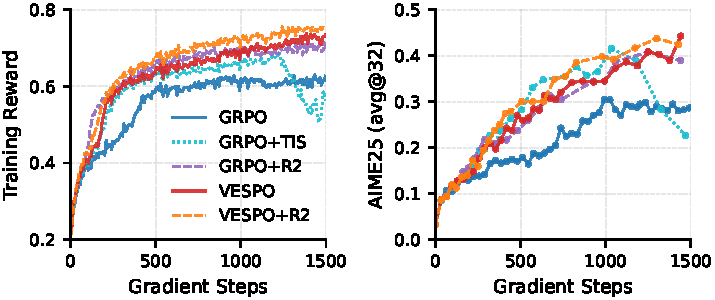
\includegraphics[width=\columnwidth]{figures/train_inference_mismatch.pdf}
  \caption{在Qwen3-30B-A3B-Base上，训练-推理不匹配下的训练稳定性。VESPO在无需特殊调整的情况下保持了稳定的训练；将VESPO与R2结合可达到最佳性能。}
  \label{fig:train-infer-mismatch}
  \vspace{-1.0em}
\end{figure}


A key design choice in VESPO is operating at the sequence level \emph{without} length normalization.
Methods like GSPO normalize importance weights by $1/T$  (sequence length) to reduce variance, but we hypothesize this creates a length bias that destabilizes training.
To test this, we compare VESPO with two normalized variants: VESPO$_{\text{sqrt}}$  (normalize by $\sqrt{T}$ ) and VESPO$_{\text{lin}}$  (normalize by $T$ ).

VESPO中的一个关键设计选择是在序列层面进行操作，\emph{不进行}长度规范化。
像GSPO这样的方法会通过$1/T$（序列长度）规范化重要性权重以降低方差，但我们假设这会产生长度偏差，从而使训练不稳定。
为了验证这一点，我们将VESPO与两种规范化变体进行比较：VESPO$_{\text{sqrt}}$（通过$\sqrt{T}$进行规范化）和VESPO$_{\text{lin}}$（通过$T$进行规范化）。

\cref{fig:ablation-length-norm} 揭示了训练动态中的显著差异。
VESPO$_{\text{lin}}$ 展现出严重的不稳定性：在第350步左右，KL散度急剧上升，随后出现梯度爆炸和奖励崩溃。
VESPO$_{\text{sqrt}}$ 表现为中等程度的不稳定性——训练奖励在约0.58处达到饱和，并开始缓慢下降，同时伴随周期性的梯度范数峰值。
相比之下，无规范化处理的 VESPO 保持了稳定的 KL 散度、受控的梯度范数，并实现了最高的训练奖励。

这些结果验证了我们的分析：长度规范化导致更长的序列主导批量梯度（因为它们不太可能被降权），从而形成一个反馈环，使模型倾向于生成更长的输出，直至训练崩溃。VESPO在序列层面采用无需长度规范化的软塑造方法，完全避免了这种失效模式。


\begin{figure}[t]
  \centering
  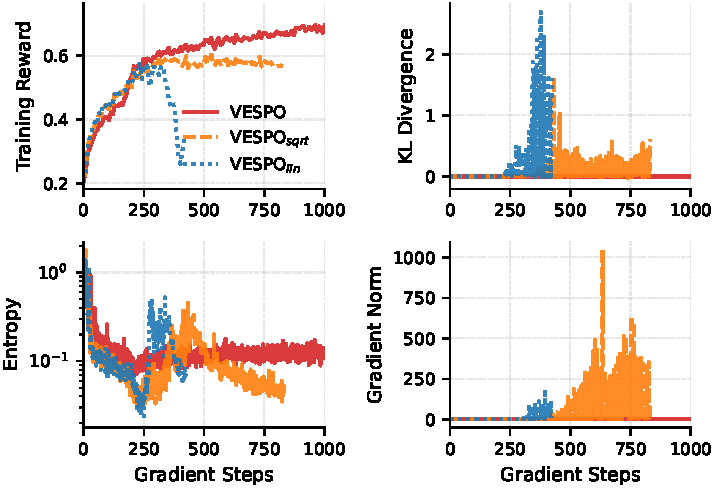
\includegraphics[width=\columnwidth]{figures/ablation_length_norm.pdf}
  \caption{长度规范化消融实验。无规范化的 VESPO 可实现稳定训练；添加 $\sqrt{T}$ 或 $T$ 规范化会导致不稳定和坍塌。}
  \label{fig:ablation-length-norm}
  \vspace{-1.2em}
\end{figure}

\subsection{消融实验：非对称超参数}
\label{sec:ablation-asymmetric}

如\cref{sec:vespo-algorithm}中所述，VESPO对正向优势和负向优势采用不同的超参数：$c^+ = (2, 3)$ 和 $c^- = (3, 2)$。  
我们通过与对称变体（\cref{fig:ablation-asymmetric}）进行对比来消融该设计。  
对正向和负向优势均使用$(2, 3)$，导致对$A < 0$的抑制不足，引发训练不稳定和奖励下降。  
对正向和负向优势均使用$(3, 2)$，则对正向优势样本施加了过度抑制，导致学习速度变慢且最终性能略有降低。

\begin{wrapfigure}{r}{0.56\columnwidth}
  \centering
  \vspace{-1em}
  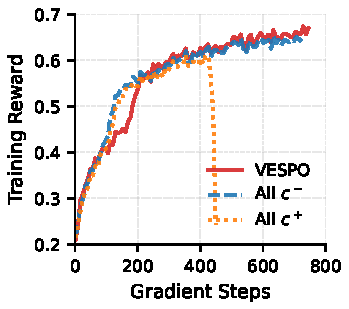
\includegraphics[width=0.56\columnwidth]{figures/ablation_asymmetric.pdf}
  \caption{对非对称超参数的消融实验。}
  \label{fig:ablation-asymmetric}
  \vspace{-.5em}
\end{wrapfigure}
非对称设计平衡了这些权衡：对负优势值施加强烈的指数抑制（$c_2 = 3$）可防止更新不稳定，而对正优势值施以较温和的抑制（$c_2 = 2$）则保留了学习信号。  
更广泛地说，我们发现只要对负优势值样本施加足够的权重下调（$W < 1$），VESPO 对适度的超参数变化具有鲁棒性。





\section{相关工作}
\label{sec:related}

\textbf{大模型的策略梯度方法。}
PPO~\citep{Schulman2017ProximalPO} 是强化学习人类反馈（RLHF）中的主流方法，采用截断的替代目标以稳定更新过程。
无价值函数的替代方法在大模型微调中逐渐受到关注：GRPO~\citep{shao2024deepseekmath} 在样本组内对奖励进行规范化，并对 token 级别比率进行截断；GSPO~\citep{Zheng2025GroupSP} 在序列层面操作，采用几何均值规范化；DAPO~\citep{yu2025dapo} 引入解耦截断与动态采样；SAPO~\citep{gao2025softadaptivepolicyoptimization} 用软自适应门控替代硬截断。
这些方法通过启发式截断或规范化来控制方差。
我们的测度变换视角揭示了它们是隐式提议分布的具体选择，而 \textbf{VESPO} 则从变分原理推导出权重函数，而非手动设计。

\textbf{强化学习中的重要性采样。}
经典的重要性采样技术——截断、自规范化、加权重要性采样——以偏差为代价实现方差减小。
在自回归大模型中，序列似然的乘积结构会放大方差，而基于 token 的重要性采样已被证明是序列级重要性采样的一阶近似~\citep{Zheng2025StabilizingRL}。
我们的视角将重要性采样塑造重新表述为测度变换，揭示出任何 $\phi(W)$ 隐式定义了一个提议分布，从而实现了原则性的变分设计。

\textbf{信任区域与裁剪。}
TRPO~\citep{Schulman2015TRPO} 通过 KL 约束来限制更新；PPO 则通过硬裁剪近似这一机制。  
当在 token 层面应用时，裁剪可能与序列级别的奖励产生冲突。  
我们的核函数提供了一种软性替代方案，能够渐进地衰减极端权重，而非突然截断。

\textbf{稳定大语言模型强化学习训练。}
近期工作通过工程解决方案应对特定的不稳定性来源：路由回放~\citep{ma2025stabilizingmoereinforcementlearning} 保证了MoE模型中专家分配的一致性；截断IS~\citep{liu-li-2025-rl-collapse} 能够检测并置零与样本不匹配的梯度。
VESPO 提供了一种互补的算法方法，可与这些技术结合使用以获得进一步提升。


\section{结论}
\label{sec:conclusion}

我们引入了一种测度变换视角，揭示了任意重要性权重变换隐式定义了一个提议分布。这一洞察使得能够建立一种有原则的变分公式，从期望的分布特性中推导出闭式重塑核。由此产生的算法 VESPO 在序列级重要性权重上运行，无需长度规范化，既保留了词元间的依赖关系，又避免了现有方法中存在的长度相关偏差。实验表明，在停滞比率高达 $64\times$ 以及完全异步训练条件下，训练过程均表现出稳定性能，并在稠密模型和 MoE 架构上均取得一致改进，尤其在训练稳定性更具挑战性的 MoE 模型上表现尤为突出。展望未来，我们看到了几个有前景的研究方向：扩展至更大规模的异步集群、推广至包含多轮交互与工具使用的智能体强化学习情景，以及将该框架应用于同策略蒸馏与离线训练。
















































































\section*{影响声明}

本文提出的研究旨在推动机器学习领域的发展。具体而言，我们提出了一种系统性方法，以在异策略条件下稳定大型语言模型的强化学习。尽管改进的强化学习训练方法可能加速更强大语言模型的开发，但我们认为其带来的社会影响不会超出语言模型能力整体提升所固有的负面效应。我们的工作可能带来多种社会后果，但其中并无需要在此特别强调的。





\bibliography{example_paper}
\bibliographystyle{icml2026}

\newpage
\appendix
\onecolumn

\begin{center}
  {\Large\bfseries VESPO：变分序列级软策略最优化 \\ 补充材料}
\end{center}
\vspace{1em}

\noindent\textbf{目录}
\vspace{0.3em}
\hrule  
\vspace{0.5em}
\noindent
\hyperref[app:implicit-proposals]{\ref{app:implicit-proposals}\hspace{1em}Implicit Proposal Distributions of Existing Methods\dotfill\pageref{app:implicit-proposals}}\\[0.3em]  
\hyperref[app:variational-derivation]{\ref{app:variational-derivation}\hspace{1em}Derivation of the Proposal Distribution\dotfill\pageref{app:variational-derivation}}\\[0.3em]  
\hyperref[app:length-normalization]{\ref{app:length-normalization}\hspace{1em}Length Normalization Introduces Bias\dotfill\pageref{app:length-normalization}}\\[0.3em]  
\hyperref[app:failure-modes]{\ref{app:failure-modes}\hspace{1em}Additional Analysis of Baseline Failure Modes\dotfill\pageref{app:failure-modes}}\\[0.3em]  
\hyperref[app:algorithm]{\ref{app:algorithm}\hspace{1em}Algorithm Pseudocode\dotfill\pageref{app:algorithm}}\\[0.3em]
\hyperref[app:hyperparameters]{\ref{app:hyperparameters}\hspace{1em}Training Hyperparameters\dotfill\pageref{app:hyperparameters}}
\vspace{0.5em}
\hrule  
\vspace{1.5em}

\section{现有方法的隐式提议分布}
\label{app:implicit-proposals}

我们分析了在 \cref{sec:measure-change} 的测度变换框架下，现有重塑策略所隐含的提议分布。

\paragraph{令牌级方法（GRPO）。}
GRPO在每个token位置独立应用裁剪，从而得到如下形式的梯度
\begin{equation}
  \nabla J_{\text{GRPO}} = \sum_{t=1}^{T} \mathbb{E}_{\tau \sim \mu}\bigl[\phi_t(\rho_t) \cdot A(\tau) \cdot \nabla \log \pi(y_t | x, y_{<t})\bigr],
\end{equation}
其中 $\phi_t(\rho_t)$  是应用于第 $t$ 个 token 比例的截断函数。  
关键观察是 \textbf{同一轨迹内的不同 token 会获得不同的权重} $\phi_t(\rho_t)$ 。  
相比之下，序列级方法为整个轨迹分配单一权重 $\phi(W)$ ：
\begin{equation}
  \nabla J_{\text{seq}} = \mathbb{E}_{\tau \sim \mu}\bigl[\phi(W) \cdot A(\tau) \cdot \sum_{t=1}^{T} \nabla \log \pi(y_t | x, y_{<t})\bigr].
\end{equation}
$Q$ 的 token-level 表示无法表示为针对任何单一提议分布 $Q$ 的重要性采样，因为这种表示要求在每个轨迹内的所有 token 梯度上具有均匀的权重。  
这种逐 token 的加权破坏了序列级别的信用分配一致性：在同一轨迹中共享相同结果的 tokens 接收到不一致的梯度信号。

\paragraph{令牌级IS作为一阶近似。}
我们现在证明，token-level IS 是 sequence-level IS 的一阶近似，遵循 \citet{Zheng2025StabilizingRL}。  
考虑未裁剪的情况，其中 $\phi_t(\rho_t) = \rho_t$ 且 $\phi(W) = W$。  
sequence-level 梯度（为清晰起见，省略优势项）为
\begin{equation}
  \nabla J_{\text{seq}} = \mathbb{E}_{\tau \sim \mu}\Bigl[W \cdot \sum_{t=1}^{T} \nabla \log \pi(y_t | \cdot)\Bigr] = \mathbb{E}_{\tau \sim \mu}\Bigl[\prod_{s=1}^{T} \rho_s \cdot \sum_{t=1}^{T} \nabla \log \pi(y_t | \cdot)\Bigr].
\end{equation}
当 $\rho_t \approx 1$ 对所有 $t$ 成立时（近同策略），我们可以通过泰勒级数展开 $W = \prod_s \rho_s$：
\begin{equation}
  W = \prod_{s=1}^{T} \rho_s \approx 1 + \sum_{s=1}^{T} (\rho_s - 1) + \sum_{s < s'} (\rho_s - 1)(\rho_{s'} - 1) + \cdots
\end{equation}
代入梯度并只保留关于 $(\rho_s - 1)$ 的一阶项：
\begin{align}
  \nabla J_{\text{seq}} & \approx \mathbb{E}_{\tau \sim \mu}\Bigl[\Bigl(1 + \sum_{s=1}^{T} (\rho_s {-} 1)\Bigr) \sum_{t=1}^{T} \nabla \log \pi(y_t | \cdot)\Bigr]                                                                                                                                     \\
                        & = \underbrace{\mathbb{E}_{\tau \sim \mu}\Bigl[\sum_{t=1}^{T} \nabla \log \pi(y_t | \cdot)\Bigr]}_{\text{REINFORCE (no IS)}} + \underbrace{\sum_{s,t} \mathbb{E}_{\tau \sim \mu}\bigl[(\rho_s {-} 1) \nabla \log \pi(y_t | \cdot)\bigr]}_{\text{first-order IS correction}}.
\end{align}
token级别的梯度是
\begin{equation}
  \nabla J_{\text{tok}} = \sum_{t=1}^{T} \mathbb{E}_{\tau \sim \mu}\bigl[\rho_t \cdot \nabla \log \pi(y_t | \cdot)\bigr] = \mathbb{E}_{\tau \sim \mu}\Bigl[\sum_{t=1}^{T} \nabla \log \pi(y_t | \cdot)\Bigr] + \sum_{t=1}^{T} \mathbb{E}_{\tau \sim \mu}\bigl[(\rho_t {-} 1) \nabla \log \pi(y_t | \cdot)\bigr].
\end{equation}
比较可知，token 级别的 IS \textbf{仅保留了一阶修正的对角项} $(s = t)$ ，忽略了其中的跨 token 相互作用 $s \neq t$ 。近似误差为
\begin{equation}
  \label{eq:token-approx-error}
  \nabla J_{\text{seq}} - \nabla J_{\text{tok}} \approx \sum_{s \neq t} \mathbb{E}_{\tau \sim \mu}\bigl[(\rho_s - 1) \nabla \log \pi(y_t | \cdot)\bigr] + O\bigl((\rho - 1)^2\bigr).
\end{equation}
此错误捕捉到了在位置 $s$ 改变策略会影响位置 $t$ 处梯度重要性的事实——一种分 token 的方法所忽略的跨 token 依赖。

\begin{remark}[When Token-Level Approximation is Reasonable]
  近似 $\nabla J_{\text{tok}} \approx \nabla J_{\text{seq}}$ 在以下情况下是合理的：
  \begin{enumerate}[itemsep=0pt, topsep=2pt]
    \item \textbf{近同策略}: $\rho_t \approx 1$ 对所有 $t$ 成立，因此高阶项和跨 token 项较小。
    \item \textbf{短序列}: 跨 token 对的数量 $(s, t)$ 与 $s \neq t$  较少，意味着累积误差更小。
  \end{enumerate}
  在实践中，大模型的强化学习通常同时违反这两个条件：异策略更新很常见，而推理任务又需要长序列。这促使了保持重要性权重完整乘积结构的序列级方法的发展。
\end{remark}

\paragraph{长度规范化（GSPO）}
GSPO 使用几何平均 $\phi(W) = W^{1/T}$，这导致提议分布显式地依赖于序列长度：
\begin{equation}
  Q_{\text{GSPO}}(\tau) \propto \mu(\tau)^{1-1/T} \cdot \pi(\tau)^{1/T}.
\end{equation}
如 $T \to \infty$、$Q_{\text{GSPO}} \to \mu$ 所示，较长的序列会趋向于获得微不足道的目标策略修正。有关由此引入的长度相关偏差的详细分析，请参见 \cref{app:length-normalization}。

\paragraph{序列级别的硬裁剪。}
如果在序列级别应用硬截断（在阈值 $c$ 处截断 $W$），则重塑函数将为 $\phi(W) = \min(W, c)$，从而引起
\begin{equation}
  Q_{\text{clip}}(\tau) \propto \min\bigl(\pi(\tau), c \cdot \mu(\tau)\bigr).
\end{equation}
这是一个\emph{截断分布}：具有$W > c$ 的轨迹被截断，而不是按成比例加权。  
在训练过程中，当轨迹跨越边界时，$W = c$ 处的不连续性可能导致最优化困难。  
请注意，标准PPO在token层面而非序列层面进行截断，因此同时结合了token层面加权和硬截断的问题。


\section{提议分布的推导}
\label{app:variational-derivation}

我们推导了 \cref{eq:constrained-opt} 中约束优化问题的闭式解。

\begin{proposition}[Solution to the Constrained Problem]
  \label{prop:proposal-solution}
  解决方法是
  \begin{align}
    \min_{Q} \;    & (1-\alpha) \, D_{\mathrm{KL}}(Q \| \mu) + \alpha \, D_{\mathrm{KL}}(Q \| \pi) \notag \\
    \text{s.t.} \; & \mathbb{E}_{Q}[W] \leq C, \quad \textstyle\int Q = 1
  \end{align}
  由以下公式给出
  \begin{equation}
    Q^*(\tau) = \frac{1}{Z} \mu(\tau)^{1-\alpha} \, \pi(\tau)^{\alpha} \, \exp(-\lambda W(\tau)),
  \end{equation}
  其中 $\lambda \geq 0$ 是矩约束的拉格朗日乘子，$Z$ 是规范化常数。
\end{proposition}

\begin{proof}
  此问题的拉格朗日函数为：
  \begin{align}
    \mathcal{L}(Q, \lambda, \gamma) = \; & (1{-}\alpha) D_{\mathrm{KL}}(Q \| \mu) + \alpha D_{\mathrm{KL}}(Q \| \pi) \notag     \\
                                         & + \lambda \bigl(\mathbb{E}_Q[W] - C\bigr) + \gamma \bigl(\textstyle\int Q - 1\bigr).
  \end{align}
  扩展KL散度：
  \begin{align}
    \mathcal{L} = \int Q(\tau) \bigl[ & \log Q(\tau) - (1{-}\alpha) \log \mu(\tau) \notag                      \\
                                      & - \alpha \log \pi(\tau) + \lambda W(\tau) \bigr] d\tau + \text{const}.
  \end{align}
  对 $Q$ 取泛函导数并令其为零：
  \begin{align}
    \frac{\delta \mathcal{L}}{\delta Q} = \; & \log Q(\tau) + 1 - (1{-}\alpha) \log \mu(\tau) \notag   \\
                                             & - \alpha \log \pi(\tau) + \lambda W(\tau) + \gamma = 0.
  \end{align}
  求解 $Q$：
  \begin{align}
    \log Q^*(\tau) & = (1{-}\alpha) \log \mu(\tau) + \alpha \log \pi(\tau) - \lambda W(\tau) + \text{const} \\
    Q^*(\tau)      & \propto \mu(\tau)^{1-\alpha} \, \pi(\tau)^{\alpha} \, \exp(-\lambda W(\tau)).
  \end{align}
  使用 $W = \pi/\mu$ ：
  \begin{align}
    Q^*(\tau) & \propto \mu(\tau)^{1-\alpha} \cdot \mu(\tau)^{\alpha} \cdot W(\tau)^{\alpha} \cdot \exp(-\lambda W(\tau)) \\
              & = \mu(\tau) \cdot W(\tau)^{\alpha} \cdot \exp(-\lambda W(\tau)).
  \end{align}
  与 $Q(\tau) = \frac{1}{Z} \mu(\tau) \phi(W(\tau))$ 从 \cref{eq:proposal-def} 比较，我们识别出
  \begin{equation}
    \phi(W) = W^{\alpha} \cdot \exp(-\lambda W).
  \end{equation}
\end{proof}

\paragraph{移位形式。}
在实际应用中，我们使用平移形式 $\phi(W) = W^{c_1} \exp(c_2(1 - W))$，其满足 $\phi(1) = 1$。  
这确保了同策略样本获得单位权重。  
我们将 $(c_1, c_2)$ 视为可调超参数，从而在变分推导所暗示的具体数值之外提供灵活性。


\section{长度规范化引入偏差}
\label{app:length-normalization}

我们分析了序列级重要性采样中的长度规范化如何引入依赖于长度的偏差，从而混淆了不同的轨迹。

\paragraph{GSPO中的长度依赖性偏差}
GSPO 使用 $\phi(W) = W^{1/T}$，该方法导致提议分布显式地依赖于序列长度 $T$：
\begin{equation}
  Q_{\text{GSPO}}(\tau) \propto \mu(\tau)^{1-1/T} \cdot \pi(\tau)^{1/T}.
\end{equation}
如 $T \to \infty$、$Q_{\text{GSPO}} \to \mu$ 所示，规范化的权重收敛至 $\exp(\mathbb{E}[\log \rho_t])$，一个与特定轨迹无关的常数。  
这导致了两个基本问题：
\begin{enumerate}[itemsep=2pt, topsep=2pt]
  \item \textbf{信号衰减}: 所有权重坍缩为一个常数，失去区分能力。
  \item \textbf{不同序列的混淆}: 具有相同 token 统计量但长度不同的序列会获得相同的权重，尽管它们的真实重要性权重不同。
\end{enumerate}

\begin{proposition}[Conflation under Length Normalization]
  \label{prop:gspo-conflation}
  对于任意两个长度为 $T_1 \neq T_2$ 的序列 $\tau_1$ ， $\tau_2$ ，若 $\frac{\log W_1}{T_1} = \frac{\log W_2}{T_2}$ ，则 GSPO 分配相同的权重：$\phi_{\text{GSPO}}(W_1) = \phi_{\text{GSPO}}(W_2)$。然而，它们的真实重要性权重不同：$W_1 = e^{T_1 \bar{r}}$ 与 $W_2 = e^{T_2 \bar{r}}$ 之差对应 $\bar{r} = \frac{\log W_1}{T_1} = \frac{\log W_2}{T_2}$。
\end{proposition}

这种混淆存在问题：一段较短的适度偏离策略的序列与一段较长的严重偏离策略的序列可能会获得相同的梯度权重，尽管它们对策略梯度的贡献应有显著差异。

\paragraph{VESPO 避免了长度依赖性偏差。}
VESPO 使用 $\phi(W) = W^{c_1} \exp(c_2(1{-}W))$，且不进行任何长度规范化。
重塑函数仅依赖于序列级别的重要性权重 $W$，而不依赖于序列长度 $T$。
两个具有相同每 token 对数比平均值 $\bar{r}$ 但长度不同的序列会获得不同的权重：较长的序列具有 $W = e^{T\bar{r}}$，该值通过 $\phi$ 适当变换。
这在保留重要性权重判别能力的同时，通过软重塑核对极端权重进行指数抑制以控制方差。


\section{基准失效模式的附加分析}
\label{app:failure-modes}

本节提供了对 \cref{sec:staleness} 中讨论的失效模式的补充细节，并通过额外的可视化结果，对比展示了每个基准下的 $N{=}4$ 与 $N{=}8$。

\begin{figure}[h]
  \centering
  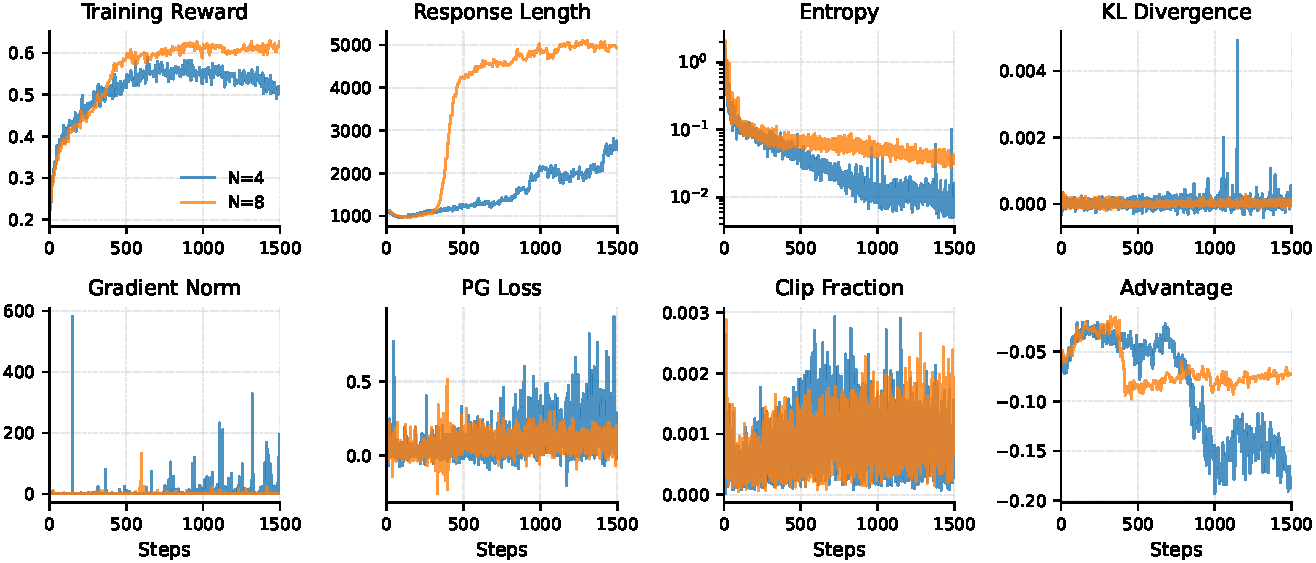
\includegraphics[width=\textwidth]{figures/grpo_n4_vs_n8_analysis.pdf}
  \caption{GRPO：$N=4$（蓝色）对比 $N=8$（橙色）。在 $N=4$ 处熵下降得更快，限制了探索。}
  \label{fig:grpo-analysis}
\end{figure}

\begin{figure}[h]
  \centering
  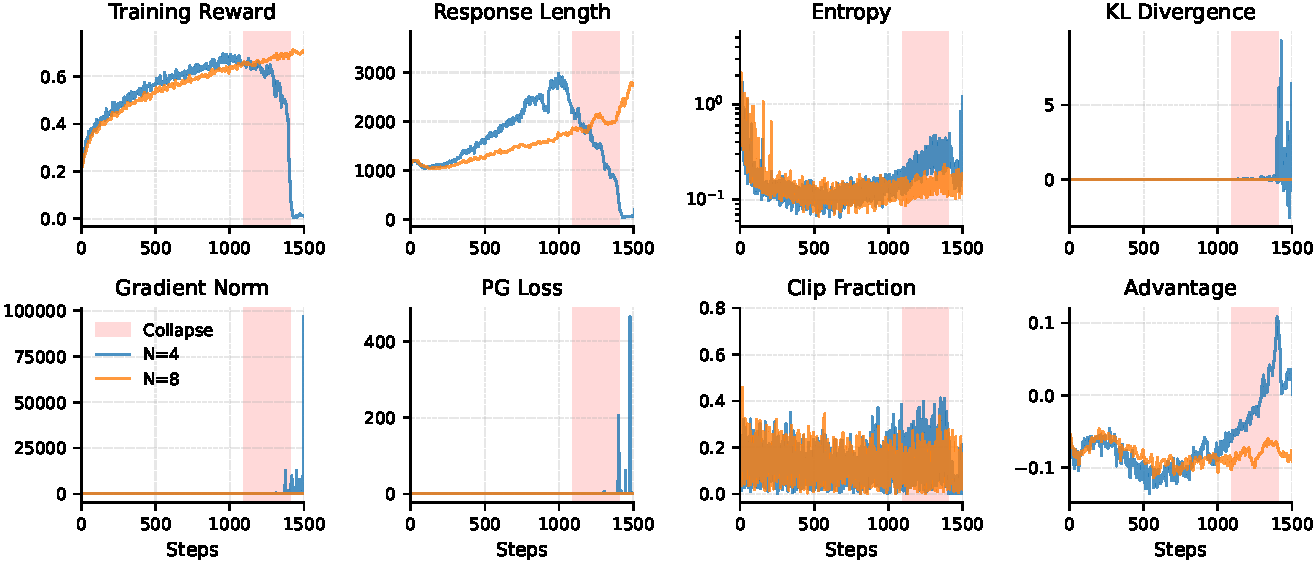
\includegraphics[width=\textwidth]{figures/gspo_collapse_analysis_4x2.pdf}
  \caption{GSPO：$N=4$（蓝色）对比 $N=8$（橙色）。响应长度增长至 ${\sim}$ 3,000 token，然后在 $N=4$ 附近于第 1,200 步左右开始坍缩。}
  \label{fig:gspo-analysis}
\end{figure}

\begin{figure}[h]
  \centering
  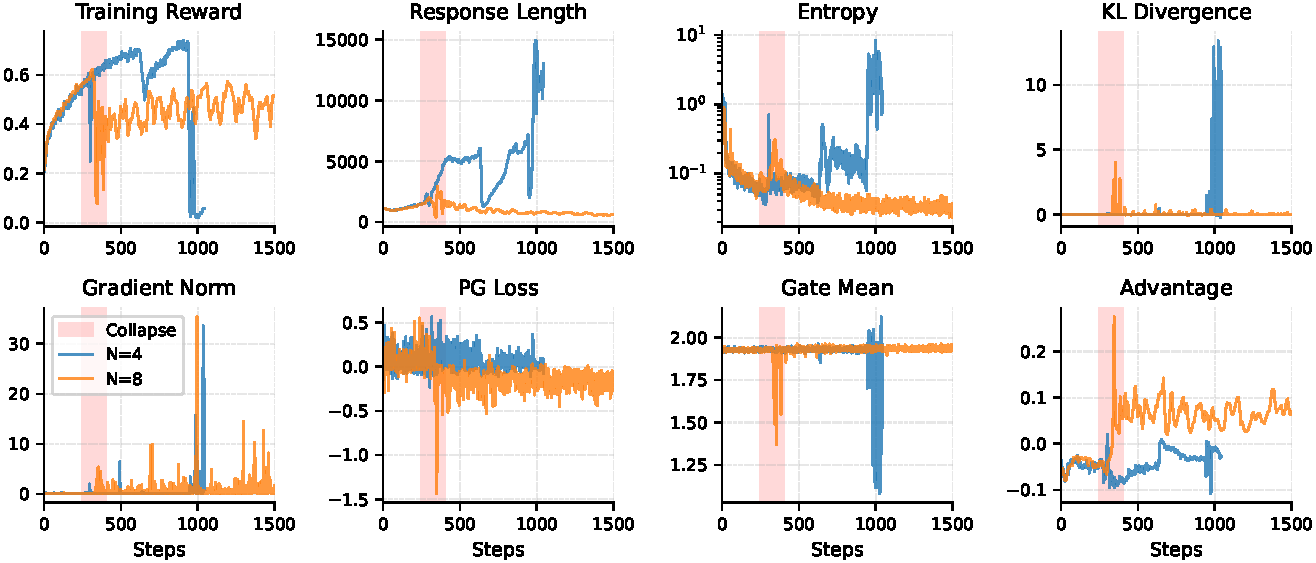
\includegraphics[width=\textwidth]{figures/sapo_n4_vs_n8_analysis.pdf}
  \caption{SAPO：$N=4$（蓝色）对比 $N=8$（橙色）。由于负优势的抑制不足，训练在 $N=8$ 处发生崩溃。}
  \label{fig:sapo-analysis}
\end{figure}


\newpage
\section{算法伪代码}
\label{app:algorithm}

\begin{lstlisting}[style=pythonstyle, title={\textbf{VESPO Policy Loss}}]
def compute_policy_loss_vespo(log_pi, log_mu, advantages, mask, c_pos, c_neg):
    """
    Args:
        log_pi: log probs from current policy, shape (batch, seq_len)
        log_mu: log probs from behavior policy, shape (batch, seq_len)
        advantages: sequence-level advantages, shape (batch,)
        mask: response mask, shape (batch, seq_len)
        c_pos: (c1, c2) for positive advantages
        c_neg: (c1, c2) for negative advantages
    """
    # Sequence-level IS ratio in log-space (true product, no length norm)
    log_ratio = log_pi - log_mu
    seq_log_w = (log_ratio * mask).sum(dim=-1)  # (batch,)
    W = exp(seq_log_w)

    # Asymmetric hyperparameter selection
    c1 = where(advantages >= 0, c_pos[0], c_neg[0])
    c2 = where(advantages >= 0, c_pos[1], c_neg[1])

    # VESPO kernel in log-space, normalized so phi(1) = 1
    log_phi = c2 + c1 * log(W) - c2 * W
    phi = exp(log_phi).detach()  # gradient scaling only

    # Policy gradient loss: grad = -phi * A * grad_log_pi
    loss = -phi.unsqueeze(-1) * advantages.unsqueeze(-1) * log_pi
    return aggregate(loss, mask)
\end{lstlisting}

\section{超参数训练}
\label{app:hyperparameters}

\cref{tab:hyperparams} 列出了所有方法共享的训练超参数。特定于方法的超参数在 \cref{sec:exp-setup} 中描述。

\begin{table}[h]
  \caption{在Qwen3-30B-A3B-Base上进行训练超参数的设置。同步与完全异步情景之间共享的参数以合并单元的形式展示。}
  \label{tab:hyperparams}
  \centering
  \setlength{\tabcolsep}{5pt}
  \begin{tabular}{@{}l|c|c@{}}
    \toprule
    \textbf{Hyperparameter}    & \textbf{Sync}                          & \textbf{Fully Async}      \\
    \midrule
    Learning rate              & \multicolumn{2}{c}{$1 \times 10^{-6}$}                             \\
    Mini-batch size (mbs)      & \multicolumn{2}{c}{256}                                            \\
    Responses per prompt       & \multicolumn{2}{c}{8}                                              \\
    Max prompt length          & \multicolumn{2}{c}{1,024}                                          \\
    Max response length        & \multicolumn{2}{c}{15,360}                                         \\
    Gradient steps             & \multicolumn{2}{c}{1,500}                                          \\
    Train temperature          & \multicolumn{2}{c}{1.0}                                            \\
    Eval temperature / top-$p$ & \multicolumn{2}{c}{1.0 / 0.7}                                      \\
    KL loss coefficient        & \multicolumn{2}{c}{0}                                              \\
    Entropy loss coefficient   & \multicolumn{2}{c}{0}                                              \\
    Training engine            & \multicolumn{2}{c}{Megatron}                                       \\
    Inference engine           & \multicolumn{2}{c}{vLLM}                                           \\
    \midrule
    Global batch size (gbs)    & $N \times 256$                         & -                         \\
    GPUs                       & 32 (colocated)                         & 48 / 16 (rollout / train) \\
    \midrule
    Parameter sync interval    & -                                      & 4                         \\
    Staleness threshold        & -                                      & 1.0                       \\
    \bottomrule
  \end{tabular}
\end{table}


\end{document}

